%% Version 4.3.2, 25 August 2014
%
%%%%%%%%%%%%%%%%%%%%%%%%%%%%%%%%%%%%%%%%%%%%%%%%%%%%%%%%%%%%%%%%%%%%%%
% Template.tex --  LaTeX-based template for submissions to the 
% American Meteorological Society
%
% Template developed by Amy Hendrickson, 2013, TeXnology Inc., 
% amyh@texnology.com, http://www.texnology.com
% following earlier work by Brian Papa, American Meteorological Society
%
% Email questions to latex@ametsoc.org.
%
%%%%%%%%%%%%%%%%%%%%%%%%%%%%%%%%%%%%%%%%%%%%%%%%%%%%%%%%%%%%%%%%%%%%%
% PREAMBLE
%%%%%%%%%%%%%%%%%%%%%%%%%%%%%%%%%%%%%%%%%%%%%%%%%%%%%%%%%%%%%%%%%%%%%

%% Start with one of the following:
% DOUBLE-SPACED VERSION FOR SUBMISSION TO THE AMS
\documentclass{ametsoc}

% TWO-COLUMN JOURNAL PAGE LAYOUT---FOR AUTHOR USE ONLY
% \documentclass[twocol]{ametsoc}

%%%%%%%%%%%%%%%%%%%%%%%%%%%%%%%%
%%% To be entered only if twocol option is used

\journal{jas}

%  Please choose a journal abbreviation to use above from the following list:
% 
%   jamc     (Journal of Applied Meteorology and Climatology)
%   jtech     (Journal of Atmospheric and Oceanic Technology)
%   jhm      (Journal of Hydrometeorology)
%   jpo     (Journal of Physical Oceanography)
%   jas      (Journal of Atmospheric Sciences)	
%   jcli      (Journal of Climate)
%   mwr      (Monthly Weather Review)
%   wcas      (Weather, Climate, and Society)
%   waf       (Weather and Forecasting)
%   bams (Bulletin of the American Meteorological Society)
%   ei    (Earth Interactions)

%%%%%%%%%%%%%%%%%%%%%%%%%%%%%%%%
%Citations should be of the form ``author year''  not ``author, year''
\bibpunct{(}{)}{;}{a}{}{,}

%%%%%%%%%%%%%%%%%%%%%%%%%%%%%%%%

%%% To be entered by author:

%% May use \\ to break lines in title:

\title{Title here}

%%% Enter authors' names, as you see in this example:
%%% Use \correspondingauthor{} and \thanks{Current Affiliation:...}
%%% immediately following the appropriate author.
%%%
%%% Note that the \correspondingauthor{} command is NECESSARY.
%%% The \thanks{} commands are OPTIONAL.

    %\authors{Author One\correspondingauthor{Author One, 
    % American Meteorological Society, 
    % 45 Beacon St., Boston, MA 02108.}
% and Author Two\thanks{Current affiliation: American Meteorological Society, 
    % 45 Beacon St., Boston, MA 02108.}}

\authors{Alexander Paterson\correspondingauthor{CGAFD, University of Exeter, Exeter, United Kingdom}}

%% Follow this form:
    % \affiliation{American Meteorological Society, 
    % Boston, Massachusetts.}

\affiliation{University of Exeter, Exeter, UK}

%% Follow this form:
    %\email{latex@ametsoc.org}

\email{ap587@exeter.ac.uk}

%% If appropriate, add additional authors, different affiliations:
    %\extraauthor{Extra Author}
    %\extraaffil{Affiliation, City, State/Province, Country}

\extraauthor{Geoffrey Vallis}
\extraaffil{University of Exeter, Exeter, UK}

%% May repeat for a additional authors/affiliations:

%\extraauthor{}
%\extraaffil{}

%%%%%%%%%%%%%%%%%%%%%%%%%%%%%%%%%%%%%%%%%%%%%%%%%%%%%%%%%%%%%%%%%%%%%
% ABSTRACT
%
% Enter your abstract here
% Abstracts should not exceed 250 words in length!
%
% For BAMS authors only: If your article requires a Capsule Summary, please place the capsule text at the end of your abstract
% and identify it as the capsule. Example: This is the end of the abstract. (Capsule Summary) This is the capsule summary. 

\abstract{Enter the text of your abstract here.}

\begin{document}

%% Necessary!
\maketitle


%%%%%%%%%%%%%%%%%%%%%%%%%%%%%%%%%%%%%%%%%%%%%%%%%%%%%%%%%%%%%%%%%%%%%
% MAIN BODY OF PAPER
%%%%%%%%%%%%%%%%%%%%%%%%%%%%%%%%%%%%%%%%%%%%%%%%%%%%%%%%%%%%%%%%%%%%%
%

%% In all cases, if there is only one entry of this type within
%% the higher level heading, use the star form: 
%%
% \section{Section title}
% \subsection*{subsection}
% text...
% \section{Section title}

%vs

% \section{Section title}
% \subsection{subsection one}
% text...
% \subsection{subsection two}
% \section{Section title}

%%%
% \section{First primary heading}

% \subsection{First secondary heading}

% \subsubsection{First tertiary heading}

% \paragraph{First quaternary heading}




\section{Introduction}






\section{Model}

We use Isca, a derivative of GFDL's FMS idealized aquaplanet model (cite model paper). Within this framework, we use a dry atmosphere forced by Newtonian relaxation to a prescribed temperature field. A new method is used to calculate an appropriate temperature field defined by simple planetary parameters. Temperatures follow a seasonal cycle prescribed by insolation derived radiative equilibrium temperatures. A tropopause height is calculated based on a radiative-convective grey atmosphere. Below the tropopause temperatures are set to follow a constant lapse rate, while above they are constant. This direct insolation temperature is used to force a flux balance equation which applies a heat capacity. 

Newtonian relaxation involves the relaxation of the model temperatures, $T$, to an equilibrium temperature, $T_{eq}$, over a relaxation timescale, $k_T$:

\begin{equation}
\label{eq:hs0}
\frac{\partial T}{\partial t} = ... -k_T(\phi,\sigma)\left[T - T_{eq}(\phi,p) \right].
\end{equation}


A diurnally averaged solar flux, $S$, is used following the derivation of \cite{Williams1997}:
\begin{equation}
\label{eq:diurnal_flux}
S(\phi) = \frac{q_0}{\pi}(H \sin\phi \sin\delta + \cos\phi \cos\delta \sin H)
\end{equation}
where $q_0$ is the bolometric solar flux. $H$ is the radian half-day length which is $0$ for perpetual night and $\pi$ for perpetual day. $\phi$ is the latitude and $\delta$ is solar declination, in the range $-\delta_0 < \delta < \delta_0$ where $\delta_0$ is the planet's obliquity.

We start with a simple radiative equilibrium model for the vertical temperature structure, determined by balance of upwards and downwards fluxes with optical depth $\tau_0$, and absorber scale height $H_a$. The vertical temperature structure then looks like:
\begin{equation}
\label{eq:vert_temp}
T^4 = U_{L,t} \left(\frac{1+\tau_0 e^{\frac{-z}{H_a}}}{2\sigma}\right)
\end{equation}
where $U_{L,t}$ is the upwards longwave radiation at the top of atmosphere, and $\sigma$ is the Stephan-Boltzmann constant. This profile features a nearly isothermal upper atmosphere, with a top of atmosphere temperature given by $T_t^4 = \frac{U_{L,t}}{2\sigma}$. The balance of albedo adjusted incoming shortwave with outgoing longwave means we can calculate this top of atmosphere temperature as:
\begin{equation}
\label{eq:toa_temp}
T_t(\phi) = \left(\frac{S(\phi)(1-A)}{2\sigma}\right)^{\frac{1}{4}}.
\end{equation}

The vertical structure is simplified into two layers: a troposphere with a uniform lapse rate, and a stratosphere with no change in temperature. The height of the boundary between these layers is determined by performing a convective adjustment to the radiative equilibrium profile, see \cite{Vallis2017}.

We assume that convection is efficient such that it establishes a convectively neutral lapse rate, $\Delta$, and that it equalizes the ground and surface layer temperatures. We can then solve numerically for the tropopause height, or use the following approximate analytic solution:
\begin{equation}
\label{eq:trop_height}
H_T(\phi) = \frac{1}{16\Gamma} \left(C T_T(\phi) + \sqrt{C^2 T_T(\phi)^2 + 32 \Gamma \tau_s H_a T_T(\phi)}\right)
\end{equation}
where $T_T$ is the tropopause/top of atmosphere temperature, C = log4, $\Gamma$ is the lapse rate, $\tau_s$ is the optical depth at the surface, and $H_a$ is the scale height of the absorber in the atmosphere (water vapour on Earth). Typical Earth values of these parameters are: $\Gamma = 6.5K km^{-1}$, $\tau_s = 5$ , and $H_a = 2 km$. The full derivation of this equation is available in \cite{GV2017} [GV2017].

We then use this height and temperature to construct a vertical equilibrium temperature profile, with constant lapse rate below the tropopause and constant temperature above.

To allow for some heat capacity, $c$, of the surface, we introduce a delay equation to the global equilibrium temperatures,
\begin{equation}
\label{eq:thermi}
c \frac{\partial T_g(\phi)}{\partial t} = \sigma \left(T_s(\phi)^4 - T_g(\phi)^4 \right).
\end{equation}

This delay is proportional to the difference in bottom layer fluxes between the previous timestep's equilibrium temperature and those calculated as described above.


\section{Results}

Obliquity only effects the seasonal distribution of incoming solar radiation. The total energy received by the planet remains constant throughout these experiments. As obliquity is increased, the planet experiences stronger seasons, until at 90 degrees obliquity where each hemisphere sees a 'polar winter' where the sun never rises for many days. Figure \ref{fig:insolation} shows the annual mean and seasonally averaged incoming solar radiation. Of note is the change from the location of peak insolation being at the equator to the poles at 54 degrees obliquity. Due to the strong seasonal effects on planets with high obliquities it is necessary to look at the seasonal rather than annual mean to avoid washing out the true behaviour. Figure \ref{fig:insolation}b) shows the mean insolation over the solstice period, defined as one month either side of the solstice. This strong effect of the polar day is clearly seen. At an obliquity of 75 degrees the insolation peaks at $xx\frac{W}{M^2}$ at the pole rather than $xx\frac{W}{m^2}$ at the equator for an Earth-like obliquity.

\begin{figure}
\label{fig:insolation}
\includegraphics[width=\textwidth]{{Figures/insolation}.png}
\caption{Top: Annual mean top of atmosphere insolation for obliquities from 15 degrees to 90 degrees. Bottom: Top of atmosphere insolation on the solstice for the same planetary obliquities.}	
\end{figure}

Now we will examine the effects of this on the basic climatology of the planet. First looking at the annual mean followed by the solstice mean for full eddy-permitting and axisymmetric models.

\begin{figure}
\label{fig:annual_mean}
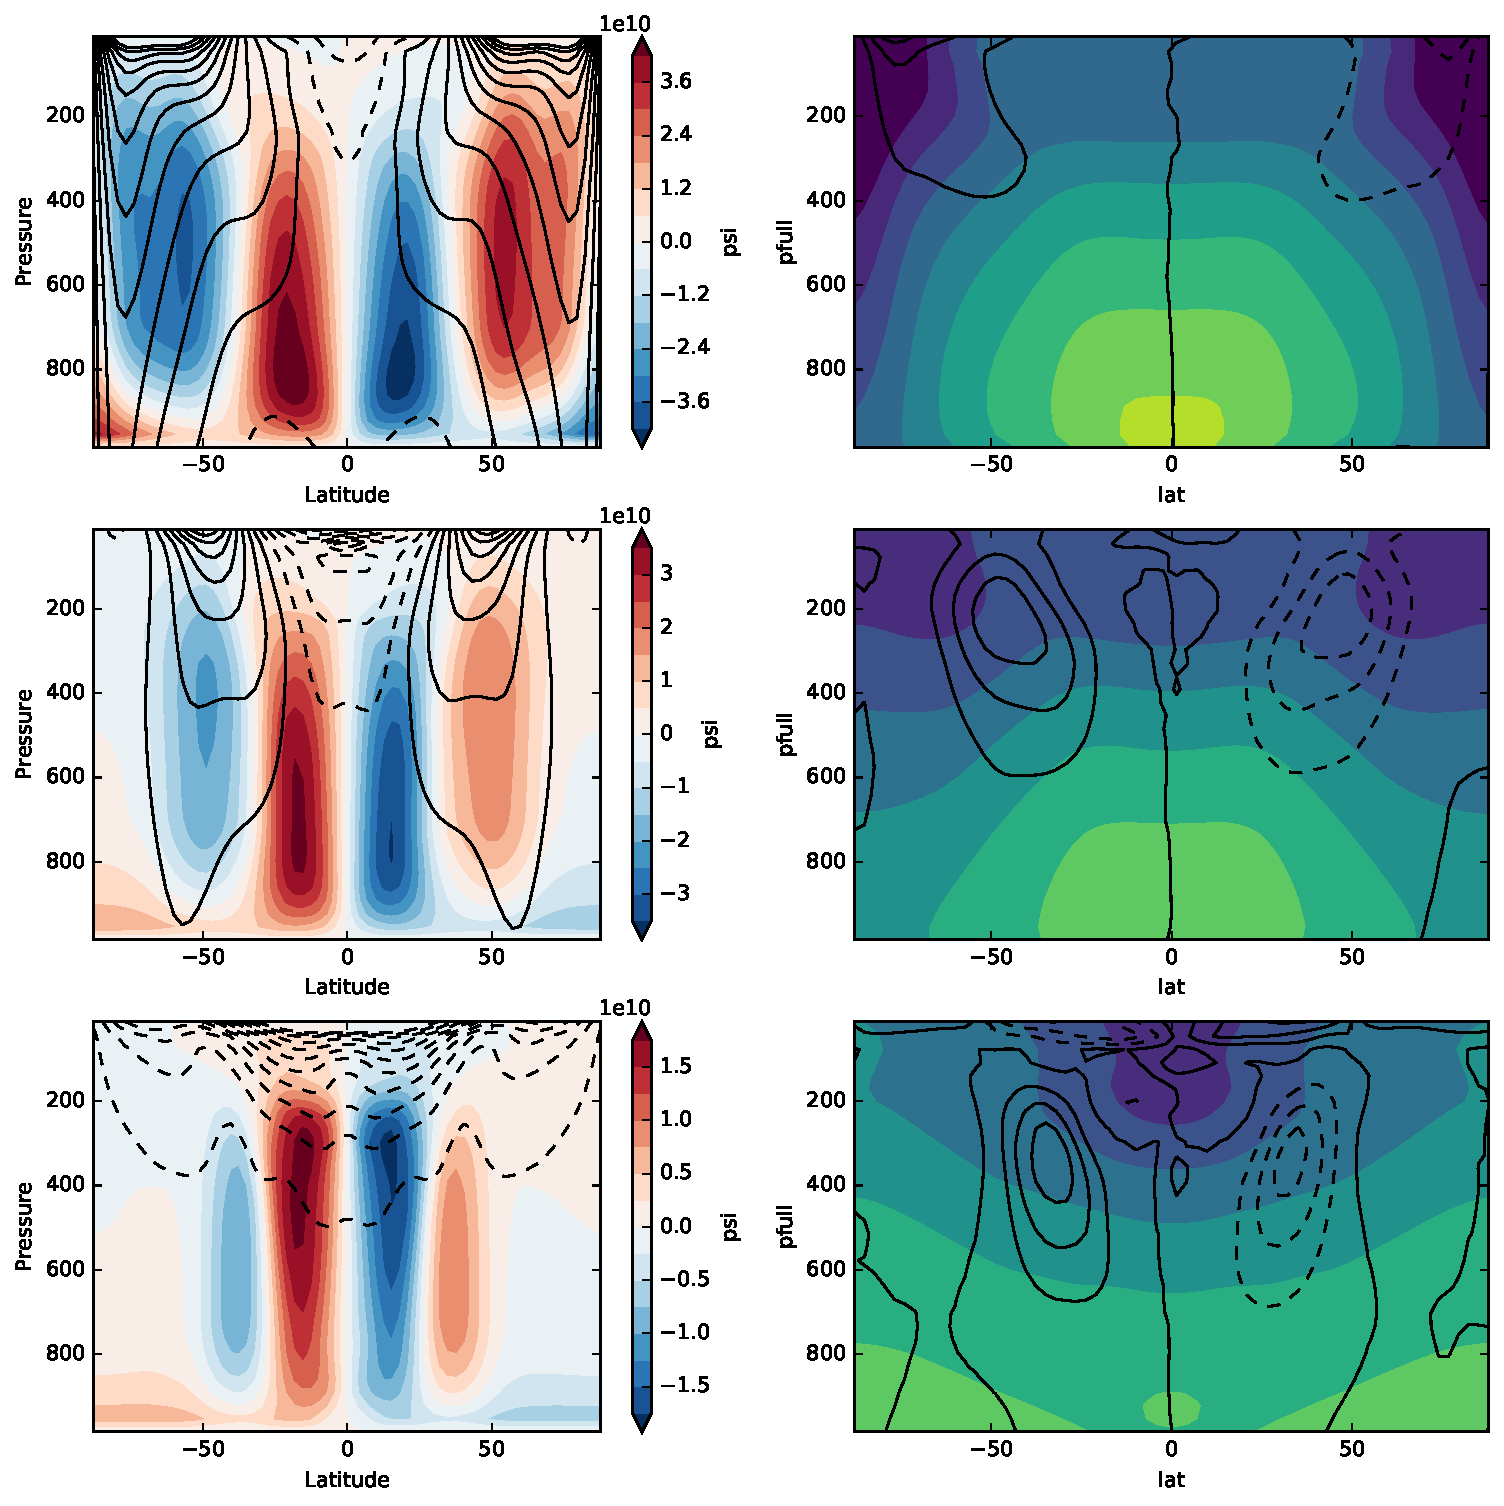
\includegraphics[width=\textwidth]{{Figures/annual_mean}.pdf}
\caption{Zonal, annual mean circulation for a series of model runs with obliquity $0^\circ$ (top), $30^\circ$ (middle) and $60^\circ$ (bottom). Left: Mass streamfunction (colours) and zonal wind (contours). Right: Temperature (colours) and meridional eddy-momentum flux, $\bar{u'v'}$ (contours).}	
\end{figure}

\begin{figure}
\label{fig:axi_annual_mean}
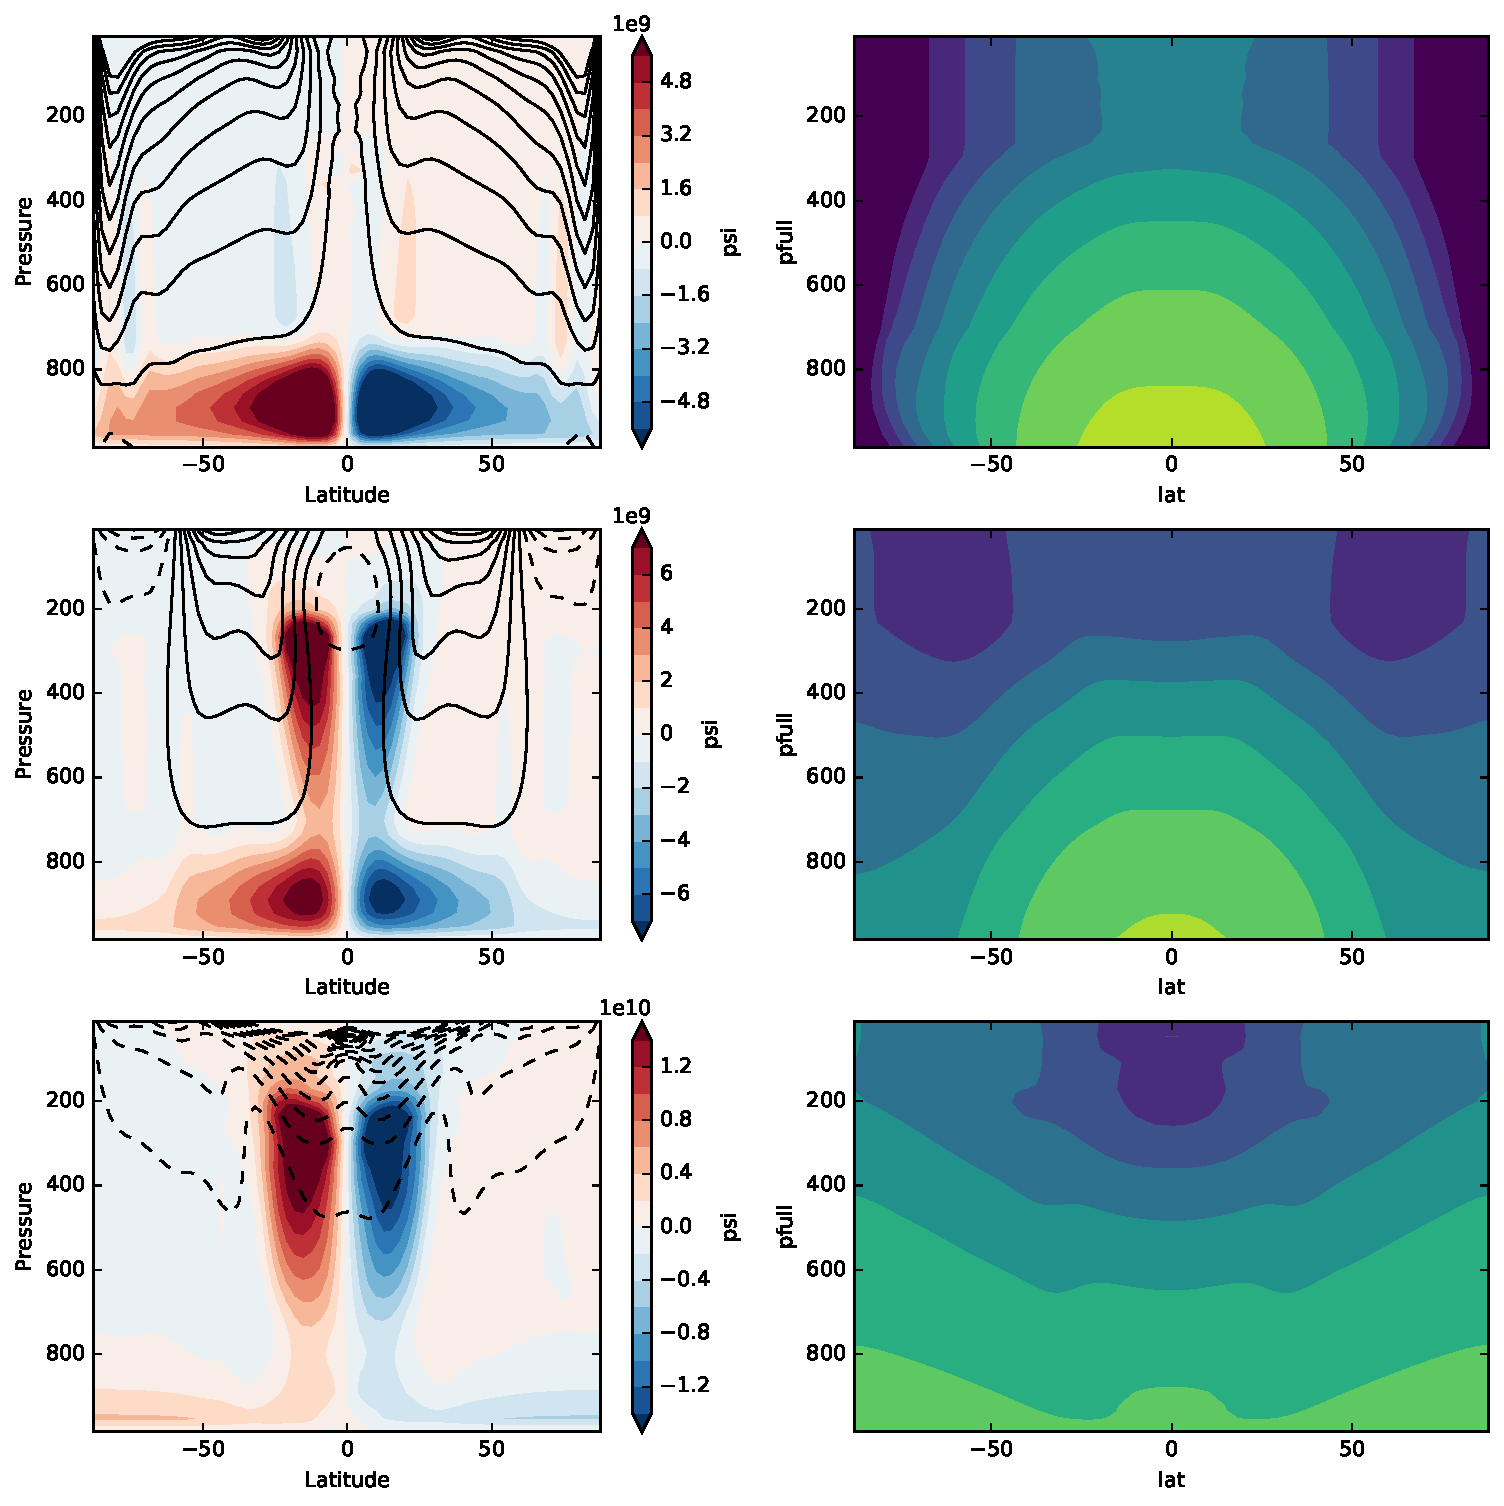
\includegraphics[width=\textwidth]{{Figures/annual_mean_axi}.pdf}
\caption{Zonal, annual mean circulation for a series of axisymmetric model runs with obliquity $0^\circ$ (top), $30^\circ$ (middle) and $60^\circ$ (bottom). Left: Mass streamfunction (colours) and zonal wind (contours). Right: Temperature (colours) and meridional eddy-momentum flux, $\bar{u'v'}$ (contours).}	
\end{figure}

At an obliquity of 30 degrees we observe a regime similar to that of the Earth (Fig: \ref{fig:annual_mean}). There is a wide equatorial region of relatively constant temperature, before dropping 20K to the poles. This temperature gradient is part of the the observed circulation structure. There are Hadley cells reach to around 30 degrees of latitude off the equator and weaker eddy-driven Ferrel cells extending from there to around 70 degrees. We also observe a small, weak polar cell in the lower atmosphere. In the zonal wind field we see a westerly jet in each hemisphere with two peaks. The first, a thermally driven jet, located higher in the troposphere and centered at the edge of the Hadley cell. The second, an eddy driven jet, in the middle of the Ferrel cell which reaches down towards the surface at approximately 60 degrees latitude. The jets are not vertically bounded as this model does not include a temperature gradient reversal in the stratosphere. 

If we increase the obliquity to 60 degrees we see a very different temperature structure. The annual mean equator-to-pole temperature gradient is reversed, and much lower as the poles are now the warmest latitudes. The lower branch of the Hadley cell has weakened compared with the lower obliquity case. The Ferrel cells have narrowed, now ending at approximately 50 degrees latitude. Overall the circulation in the annual mean is significantly weaker, the meridional mean mass overturning streamfunction is half as intense across the atmosphere. There are no westerly jets present as the strong seasonal effects are masking the jets when the annual mean is taken.

We have also run the same planet under axisymmetric conditions. Here we only allow wave number one in the spectral model, so no eddies are permitted. In this model the climate differs in a few key ways. [][][]

\begin{figure}
\label{fig:solstice_mean}
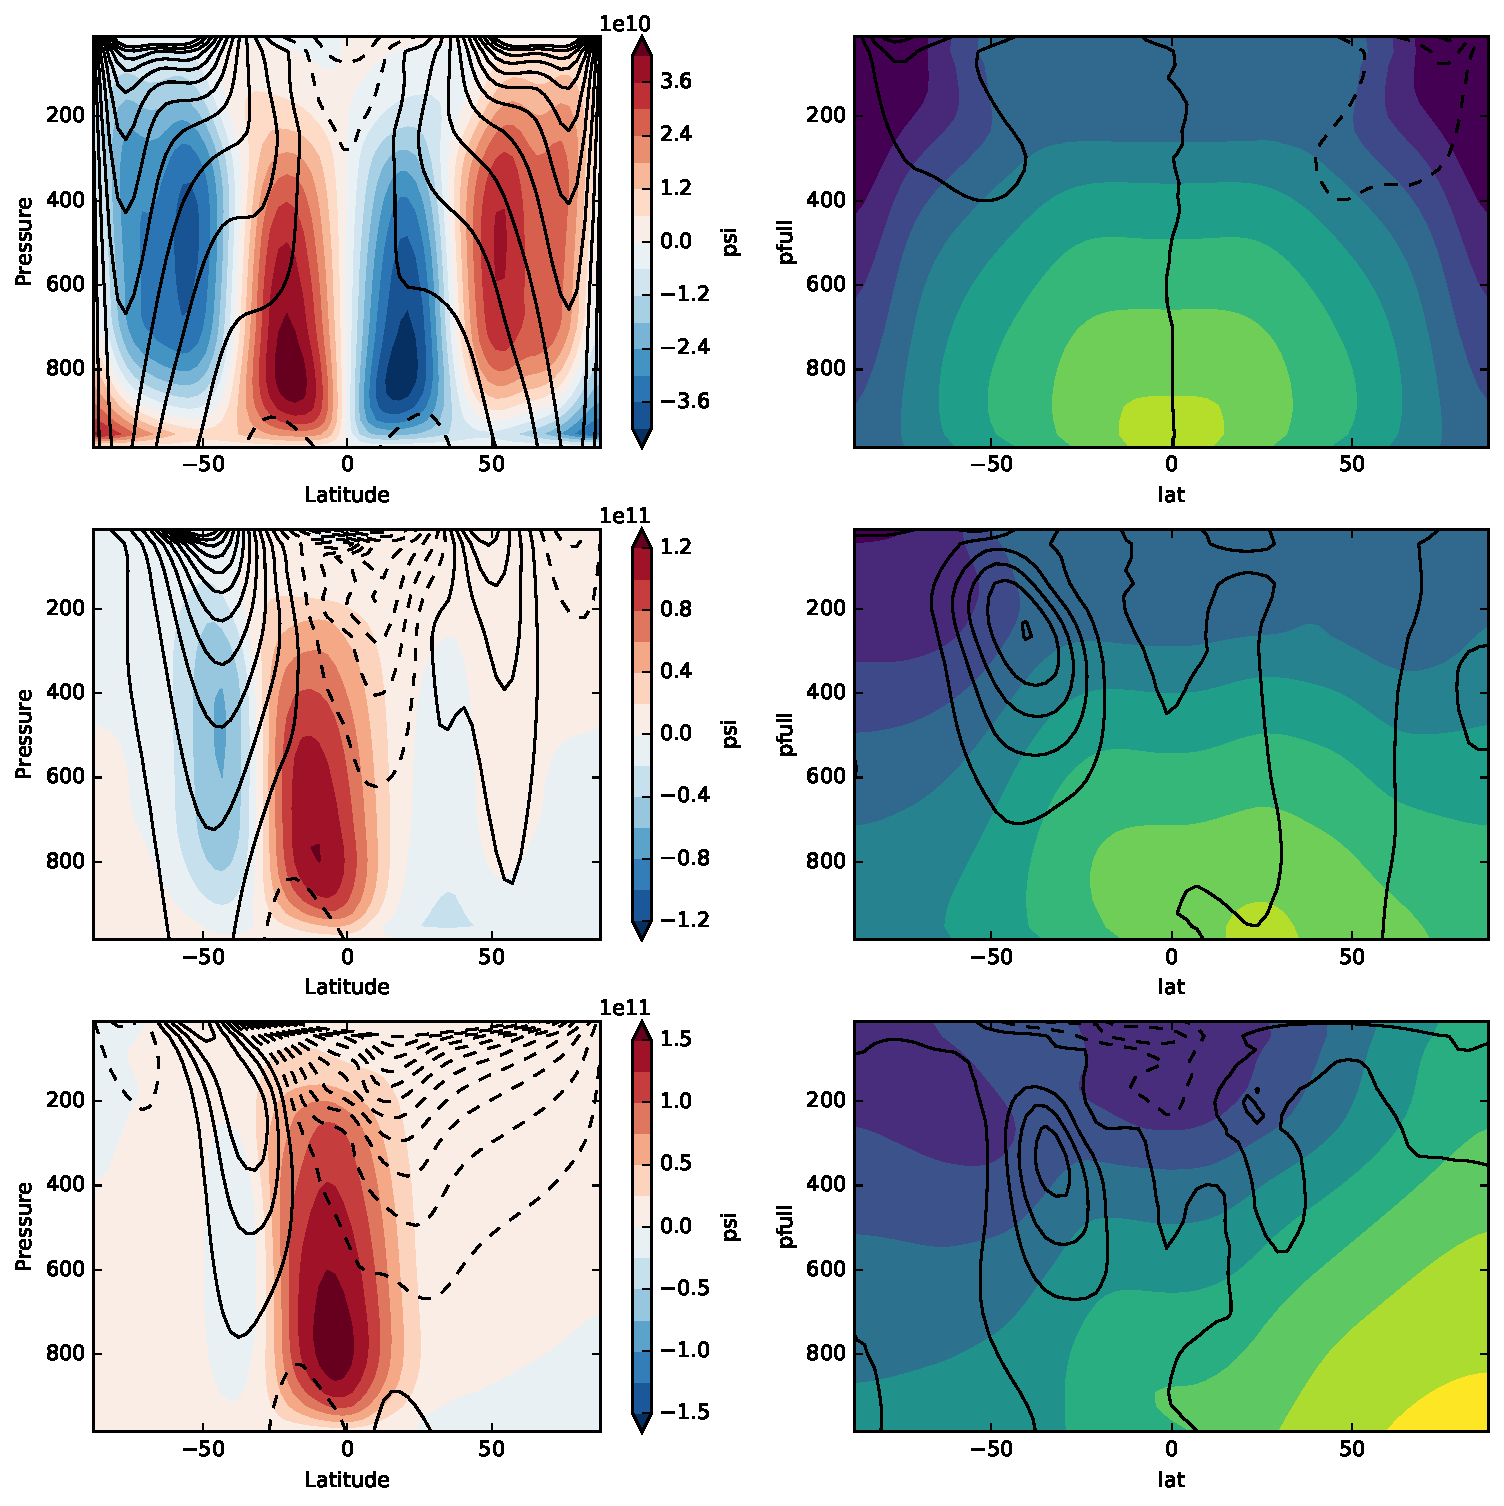
\includegraphics[width=\textwidth]{{Figures/solstice_mean}.pdf}
\caption{Zonal, solstice mean circulation for a series of model runs with obliquity $0^\circ$ (top), $30^\circ$ (middle) and $60^\circ$ (bottom). Left: Mass streamfunction (colours) and zonal wind (contours). Right: Temperature (colours) and meridional eddy-momentum flux, $\bar{u'v'}$ (contours).}	
\end{figure}

\begin{figure}
\label{fig:axi_solstice_mean}
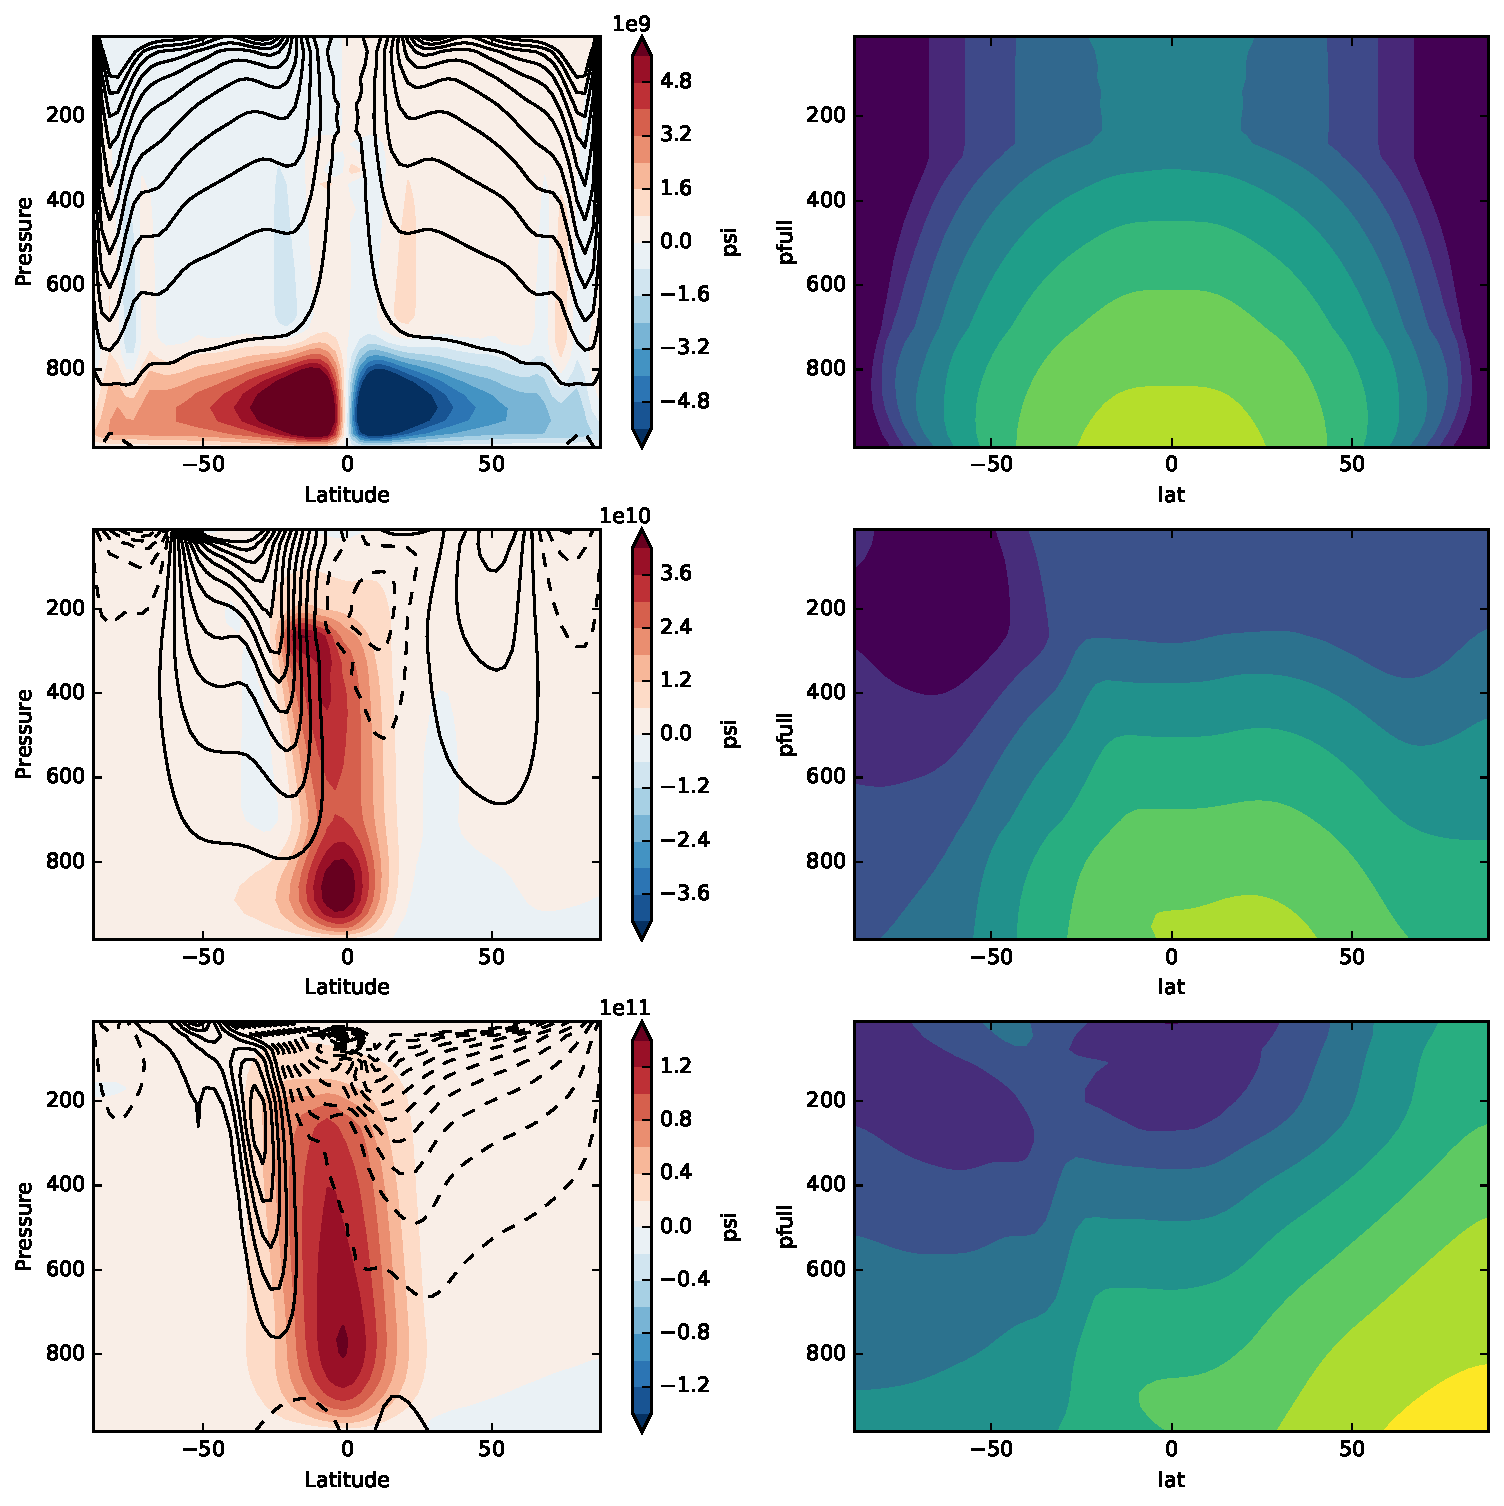
\includegraphics[width=\textwidth]{{Figures/solstice_mean_axi}.pdf}
\caption{Zonal, solstice mean circulation for a series of axisymmetric model runs with obliquity $0^\circ$ (top), $30^\circ$ (middle) and $60^\circ$ (bottom). Left: Mass streamfunction (colours) and zonal wind (contours). Right: Temperature (colours) and meridional eddy-momentum flux, $\bar{u'v'}$ (contours).} 	
\end{figure}

To actually understand how the changing obliquity is affecting the climate, we need to examine the seasonal effects in more detail. Figure \ref{fig:solstice_mean} shows the solstice mean for the experiments detailed in Figure \ref{fig:annual_mean}. The solstice period here is defined as the time period one month either side of the solstice. In our 30 degree obliquity experiment the offset heating results in a temperature field maxima offset from the equator by approximately 25 degrees. This is caused by the heat capacity of the model moderating the seasonal shift. The mass streamfunction shows a cross-equatorial winter Hadley cell paired with a very weak summer cell. The latitude of the ascending branch of the winter Hadley cell does not align with the latitude of maximum temperature; we explore the reasons behind this in section xx. The westerly jet latitudes are fairly unchanged from the annual mean case, the main difference between them being their relative strengths. The winter hemisphere jet is much stronger, associated with the strong Hadley and Ferrel cells. The 30 degree obliquity experiment produces a seasonal climate similar to that of other idealised models of Earth xx. 
At 60 degrees obliquity, Figure \ref{fig:solstice_mean}b), the temperature maxima is now located at the pole. This is consistent with predictions from the insolation equation. Past 21 degrees obliquity the insolation maxima for the season is at the pole. There is now one global circulation cell, the winter cross-equatorial Hadley cell. Interestingly it is of similar size and intensity as the Hadley cell at 30 degrees obliquity, while the temperature structure has changed significantly. We look in detail at the reasons for this in section xx. An eddy driven westerly jet is not present at higher obliquities. Instead we only see the thermally driven upper jet centered at the edge of the Hadley cell. In the summer hemisphere we see an easterly jet with a maxima on the up-welling branch of the Hadley cell. This is a thermal jet caused by the reversed, now pole-equator, temperature gradient.


\begin{figure}
\label{fig:eqpoleT}
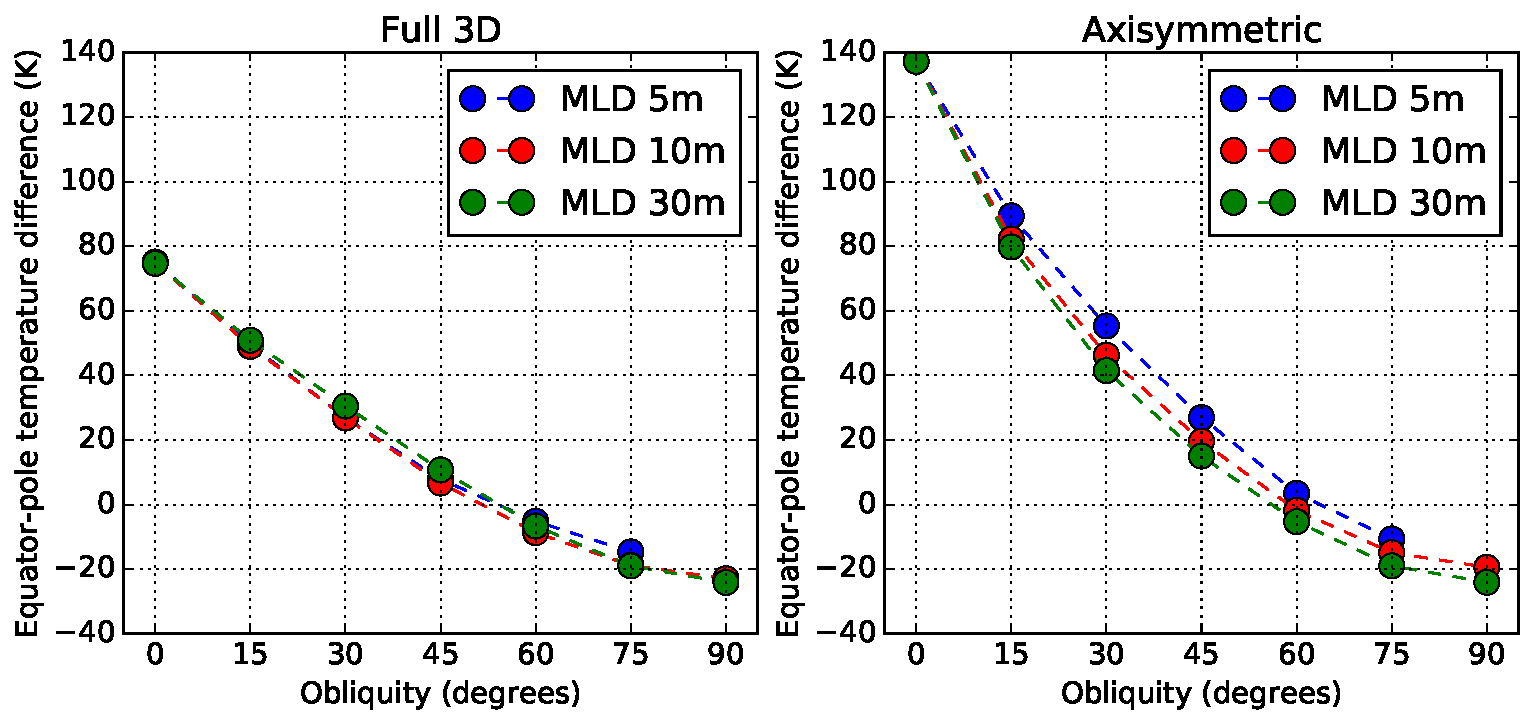
\includegraphics[width=\textwidth]{{Figures/eq-pole_temp}.pdf}
\caption{Annual mean equator-to-pole temperature difference for full 3D eddy permitting, and axisymmetric obliquity variations. Note that the temperature difference is negative for obliquities greater than around 50 degrees. Past this point the poles are warmer than the equator due to the intense polar summer.}	
\end{figure}


Figure \ref{fig:eqpoleT} shows the annual mean equator-to-pole termperature difference for eddt permitting and axisymmetric models. Both cases feature a clear negative relationship between therse valies. At smalller obliquities the axisymmetric runs have a much larger equator-to-pole difference as there are no eddies providing poleward heat transport. Past 54 degrees in the 3D case, we see a negative temperature gradient. Here the poles are warmer than the equator, as we saw in the field slices (Fig \ref{fig:solstice_mean}). At very hight obliquities, greater than 60 degrees, we see the axisymmetric model and 3D have essentially the same values. This is further evidence to the reduced role of eddies at high obliquities - with the climate dominated by a single thermally direct overturning Hadley cell.



\begin{figure}
\label{fig:AM_hadleystr}
\includegraphics[width=\textwidth]{{Figures/AM_hadley_str}.pdf}
\caption{Annual mean Hadley cell strength for mixed layer depth 5, 10, 30m.}
\end{figure}

The strength of the solstice Hadley cell is observed to increase consistently from 0 to 90 degrees obliquity. This is in constrast with the annual neab cekk whucg decreases in strength, with an exception at 30 degrees. At 30 degrees there is a strong winter cell which is still largely concentrated in the winter hemisphere. At high obliquities, this winter cell is centered over the equator, and so in the annual mean is largely cancelled out.



\begin{figure}
\label{fig:seasonal_hadleystr}
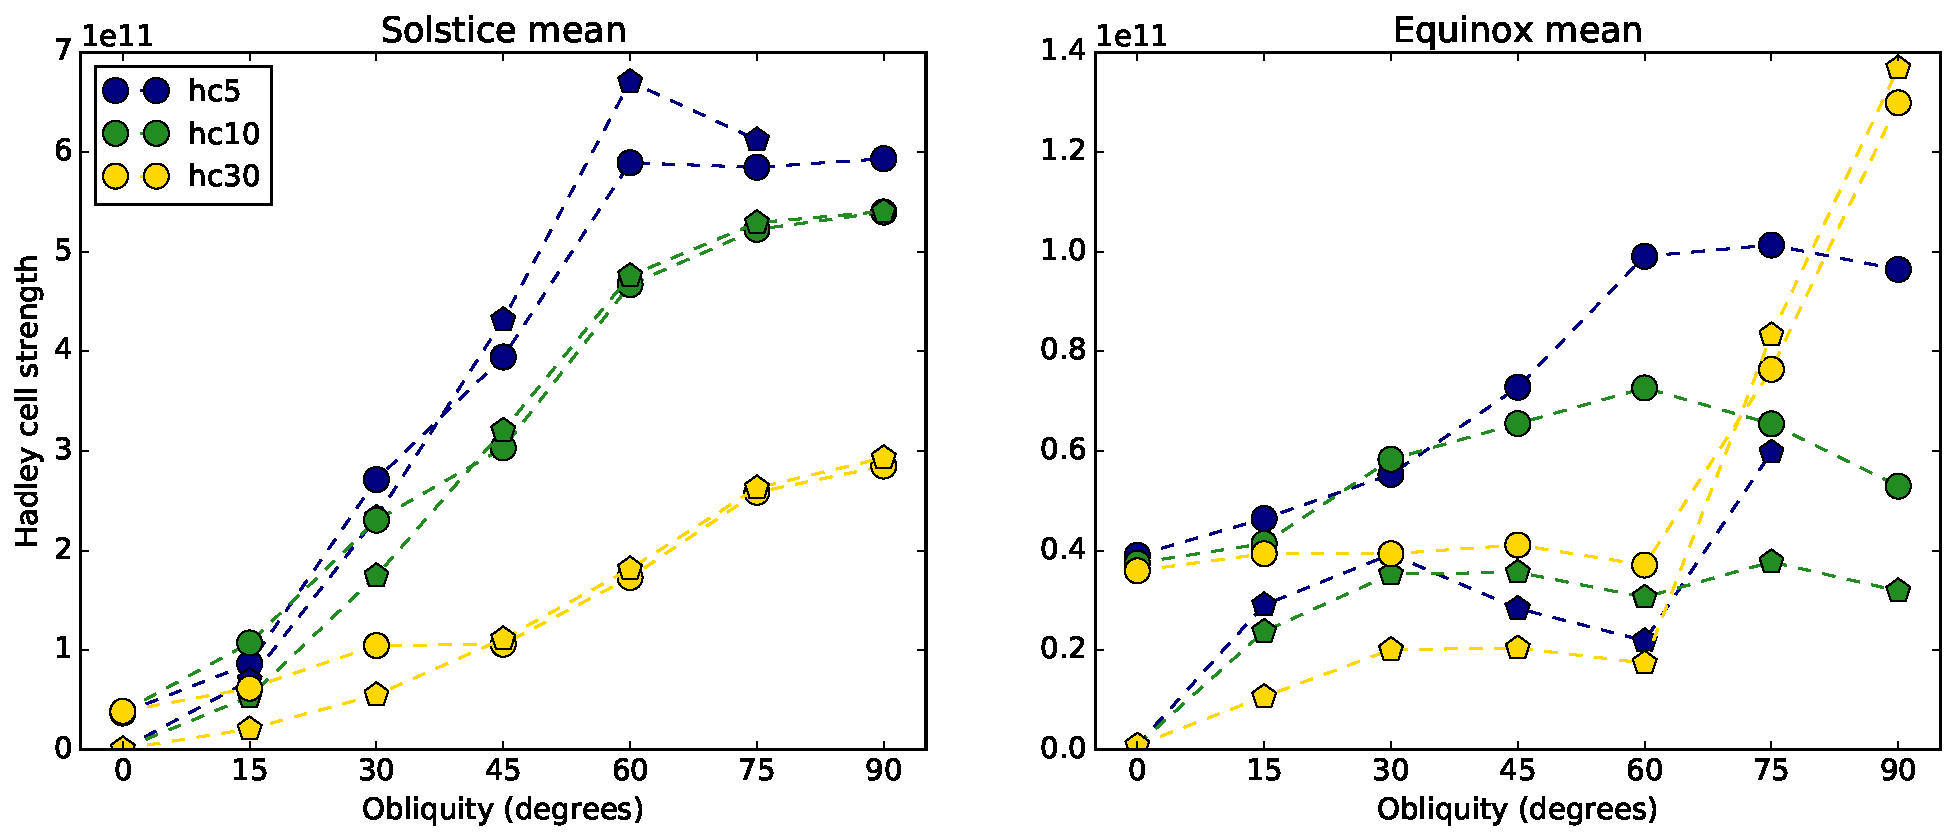
\includegraphics[width=\textwidth]{{Figures/seasonal_hadley_str}.pdf}
\caption{Strength of the winter and equinox Hadley cell for mixed layer depth 5, 10, and 30m.}
\end{figure}

\begin{figure}
\label{fig:axi_M_hadleystr}
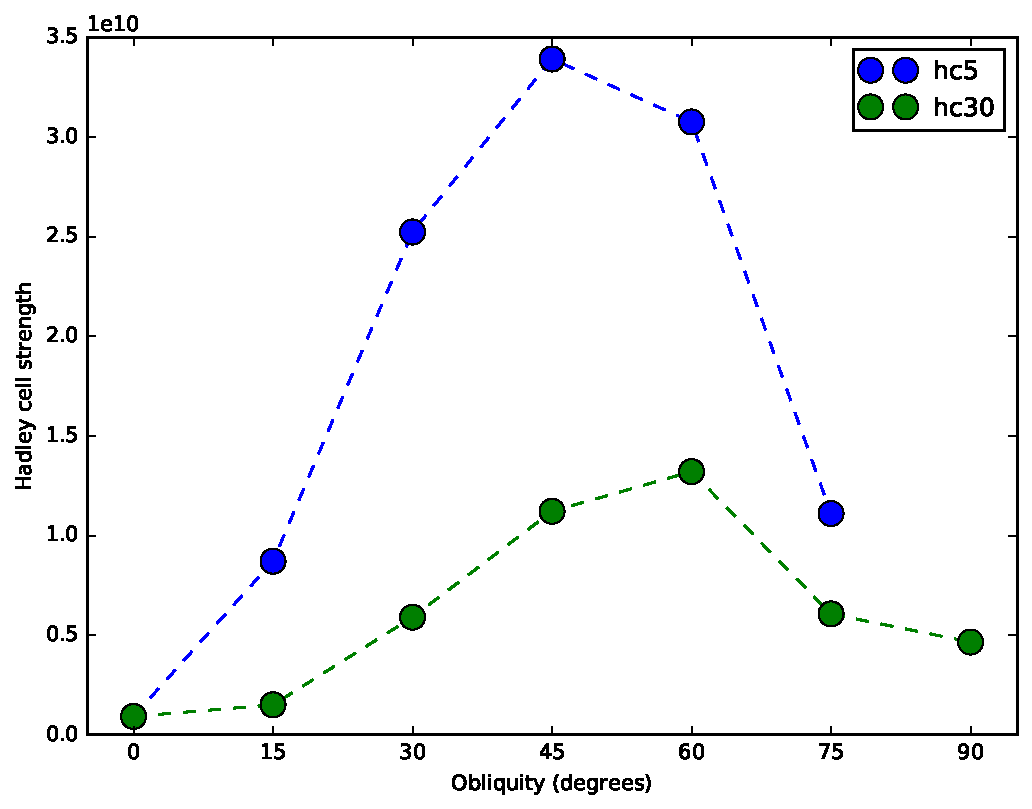
\includegraphics[width=\textwidth]{{Figures/AM_hadley_str_axi}.pdf}
\caption{Annual mean axisymmetric Hadley cell strength for mixed layer depth 5, 10, 30m.}
\end{figure}

\begin{figure}
\label{fig:itcz_v_obl}
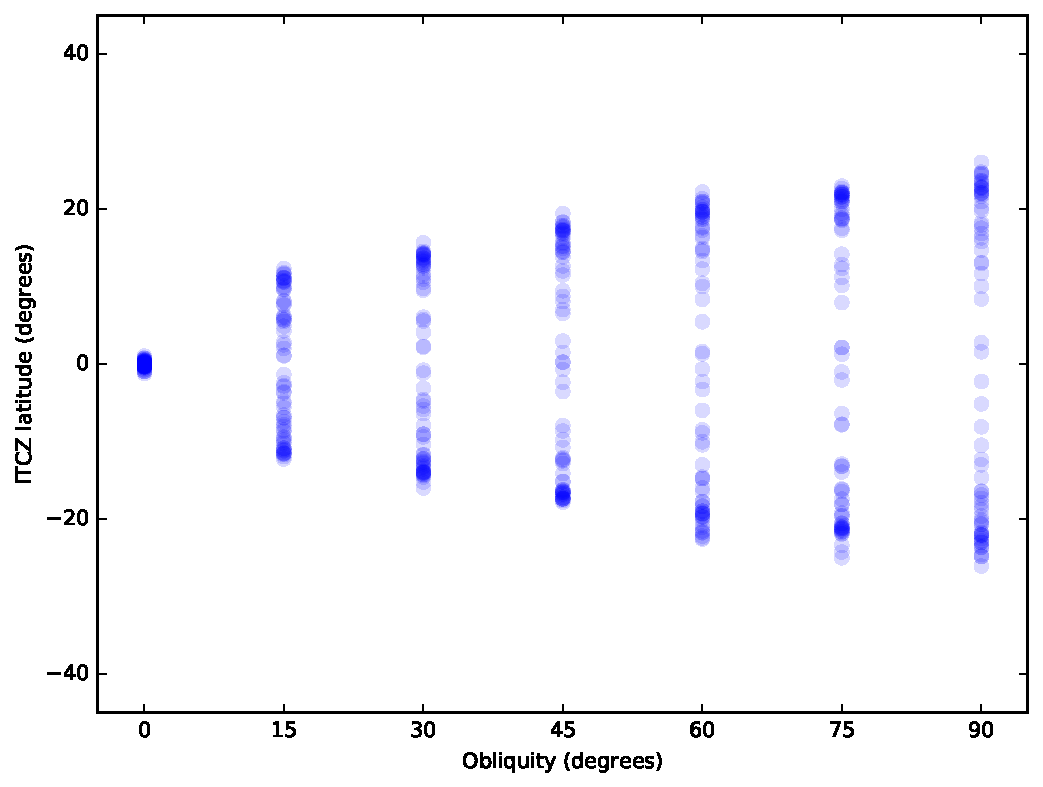
\includegraphics[width=\textwidth]{{Figures/ITCZ_lats_hc10}.pdf}
\caption{5-day mean latitude of the ITCZ for experiments with a mixed layer depth of 10m. We see a strong initial trend when obliquity is first introduced, and slow growth in the outer limit of the ITCZ for any further obliquity. This outer limit is also much less than the obliquity of the planet, only reaching 25 degrees with a 90 degree obliquity.}
\end{figure}

%\begin{figure}
%\label{fig:axi_solstice_hadleystr}
%\includegraphics[width=\textwidth]{{Figures/sol_hadley_str_axi}.pdf}
%\caption{Strength of the axisymmetric winter Hadley cell for mixed layer depth 5, 10, and 30m.}
%\end{figure}


\begin{figure}
\label{fig:temppsi}
\includegraphics[width=\textwidth]{{Figures/hc10_temp-psi_HH}.png}
\caption{Bottom level temperature (left) and 500ish hPa mass streamfunction (right) for obliquities of 0, 15, 30, 45 degrees. Overplotted are points showing the ITCZ latitude (black), model derived edge of Hadley cell (blue), and Held and Hou theoretical scaling for the Hadley cell edge (red).}	
\end{figure}


\begin{figure}
\label{fig:uvuvdy}
\includegraphics[width=\textwidth]{{Figures/hc10_uv-uvdy_HH}.png}
\caption{The same but for eddy flux and eddy flux divergence.}	
\end{figure}

%Now we examine the performance of some theoretical scaling models describing the Hadley cell strength and extent. First, the axisymmetric, equinoctial argument from Held and Hou (1980).



%%%%%%%%%%%%%%%%%%%%%%%%%%%%%%%%%%%%%%%%%%%%%%%%%%%%%%%%%%%%%%%%%%%%%
% ACKNOWLEDGMENTS
%%%%%%%%%%%%%%%%%%%%%%%%%%%%%%%%%%%%%%%%%%%%%%%%%%%%%%%%%%%%%%%%%%%%%
%
\acknowledgments
Start acknowledgments here.

%%%%%%%%%%%%%%%%%%%%%%%%%%%%%%%%%%%%%%%%%%%%%%%%%%%%%%%%%%%%%%%%%%%%%
% APPENDIXES
%%%%%%%%%%%%%%%%%%%%%%%%%%%%%%%%%%%%%%%%%%%%%%%%%%%%%%%%%%%%%%%%%%%%%
%
% Use \appendix if there is only one appendix.
%\appendix

% Use \appendix[A], \appendix}[B], if you have multiple appendixes.
%\appendix[A]

%% Appendix title is necessary! For appendix title:
%\appendixtitle{}

%%% Appendix section numbering (note, skip \section and begin with \subsection)
% \subsection{First primary heading}

% \subsubsection{First secondary heading}

% \paragraph{First tertiary heading}

%% Important!
%\appendcaption{<appendix letter and number>}{<caption>} 
%must be used for figures and tables in appendixes, e.g.,
%
%\begin{figure}
%\noindent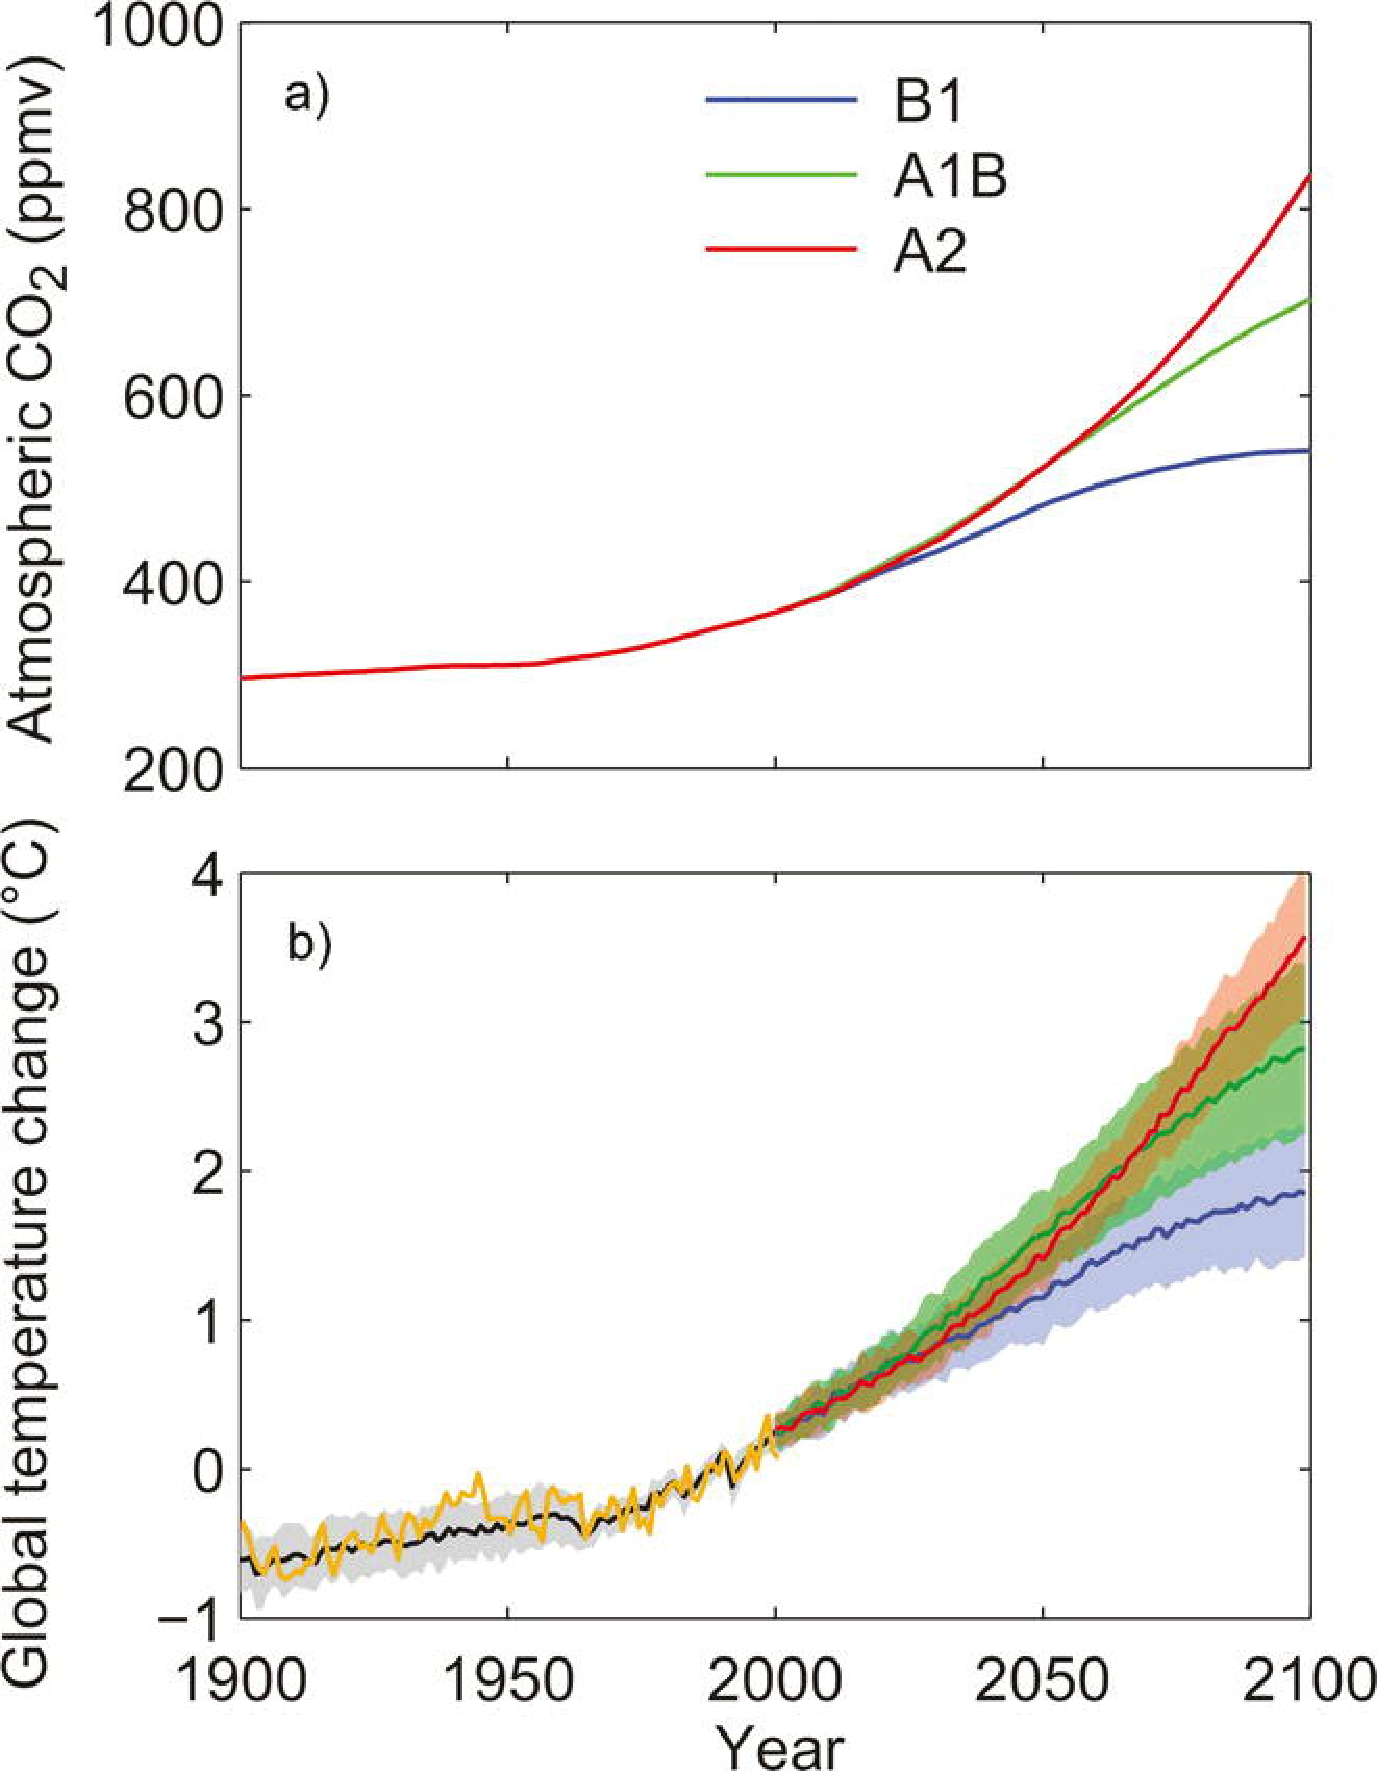
\includegraphics[width=19pc,angle=0]{figure01.pdf}\\
%\appendcaption{A1}{Caption here.}
%\end{figure}
%
% All appendix figures/tables should be placed in order AFTER the main figures/tables, i.e., tables, appendix tables, figures, appendix figures.
%
%%%%%%%%%%%%%%%%%%%%%%%%%%%%%%%%%%%%%%%%%%%%%%%%%%%%%%%%%%%%%%%%%%%%%
% REFERENCES
%%%%%%%%%%%%%%%%%%%%%%%%%%%%%%%%%%%%%%%%%%%%%%%%%%%%%%%%%%%%%%%%%%%%%
% Make your BibTeX bibliography by using these commands:
\bibliographystyle{ametsoc2014}
\bibliography{references}


%%%%%%%%%%%%%%%%%%%%%%%%%%%%%%%%%%%%%%%%%%%%%%%%%%%%%%%%%%%%%%%%%%%%%
% TABLES
%%%%%%%%%%%%%%%%%%%%%%%%%%%%%%%%%%%%%%%%%%%%%%%%%%%%%%%%%%%%%%%%%%%%%
%% Enter tables at the end of the document, before figures.
%%
%
%\begin{table}[t]
%\caption{This is a sample table caption and table layout.  Enter as many tables as
%  necessary at the end of your manuscript. Table from Lorenz (1963).}\label{t1}
%\begin{center}
%\begin{tabular}{ccccrrcrc}
%\hline\hline
%$N$ & $X$ & $Y$ & $Z$\\
%\hline
% 0000 & 0000 & 0010 & 0000 \\
% 0005 & 0004 & 0012 & 0000 \\
% 0010 & 0009 & 0020 & 0000 \\
% 0015 & 0016 & 0036 & 0002 \\
% 0020 & 0030 & 0066 & 0007 \\
% 0025 & 0054 & 0115 & 0024 \\
%\hline
%\end{tabular}
%\end{center}
%\end{table}

%%%%%%%%%%%%%%%%%%%%%%%%%%%%%%%%%%%%%%%%%%%%%%%%%%%%%%%%%%%%%%%%%%%%%
% FIGURES
%%%%%%%%%%%%%%%%%%%%%%%%%%%%%%%%%%%%%%%%%%%%%%%%%%%%%%%%%%%%%%%%%%%%%
%% Enter figures at the end of the document, after tables.
%%
%
%\begin{figure}[t]
%  \noindent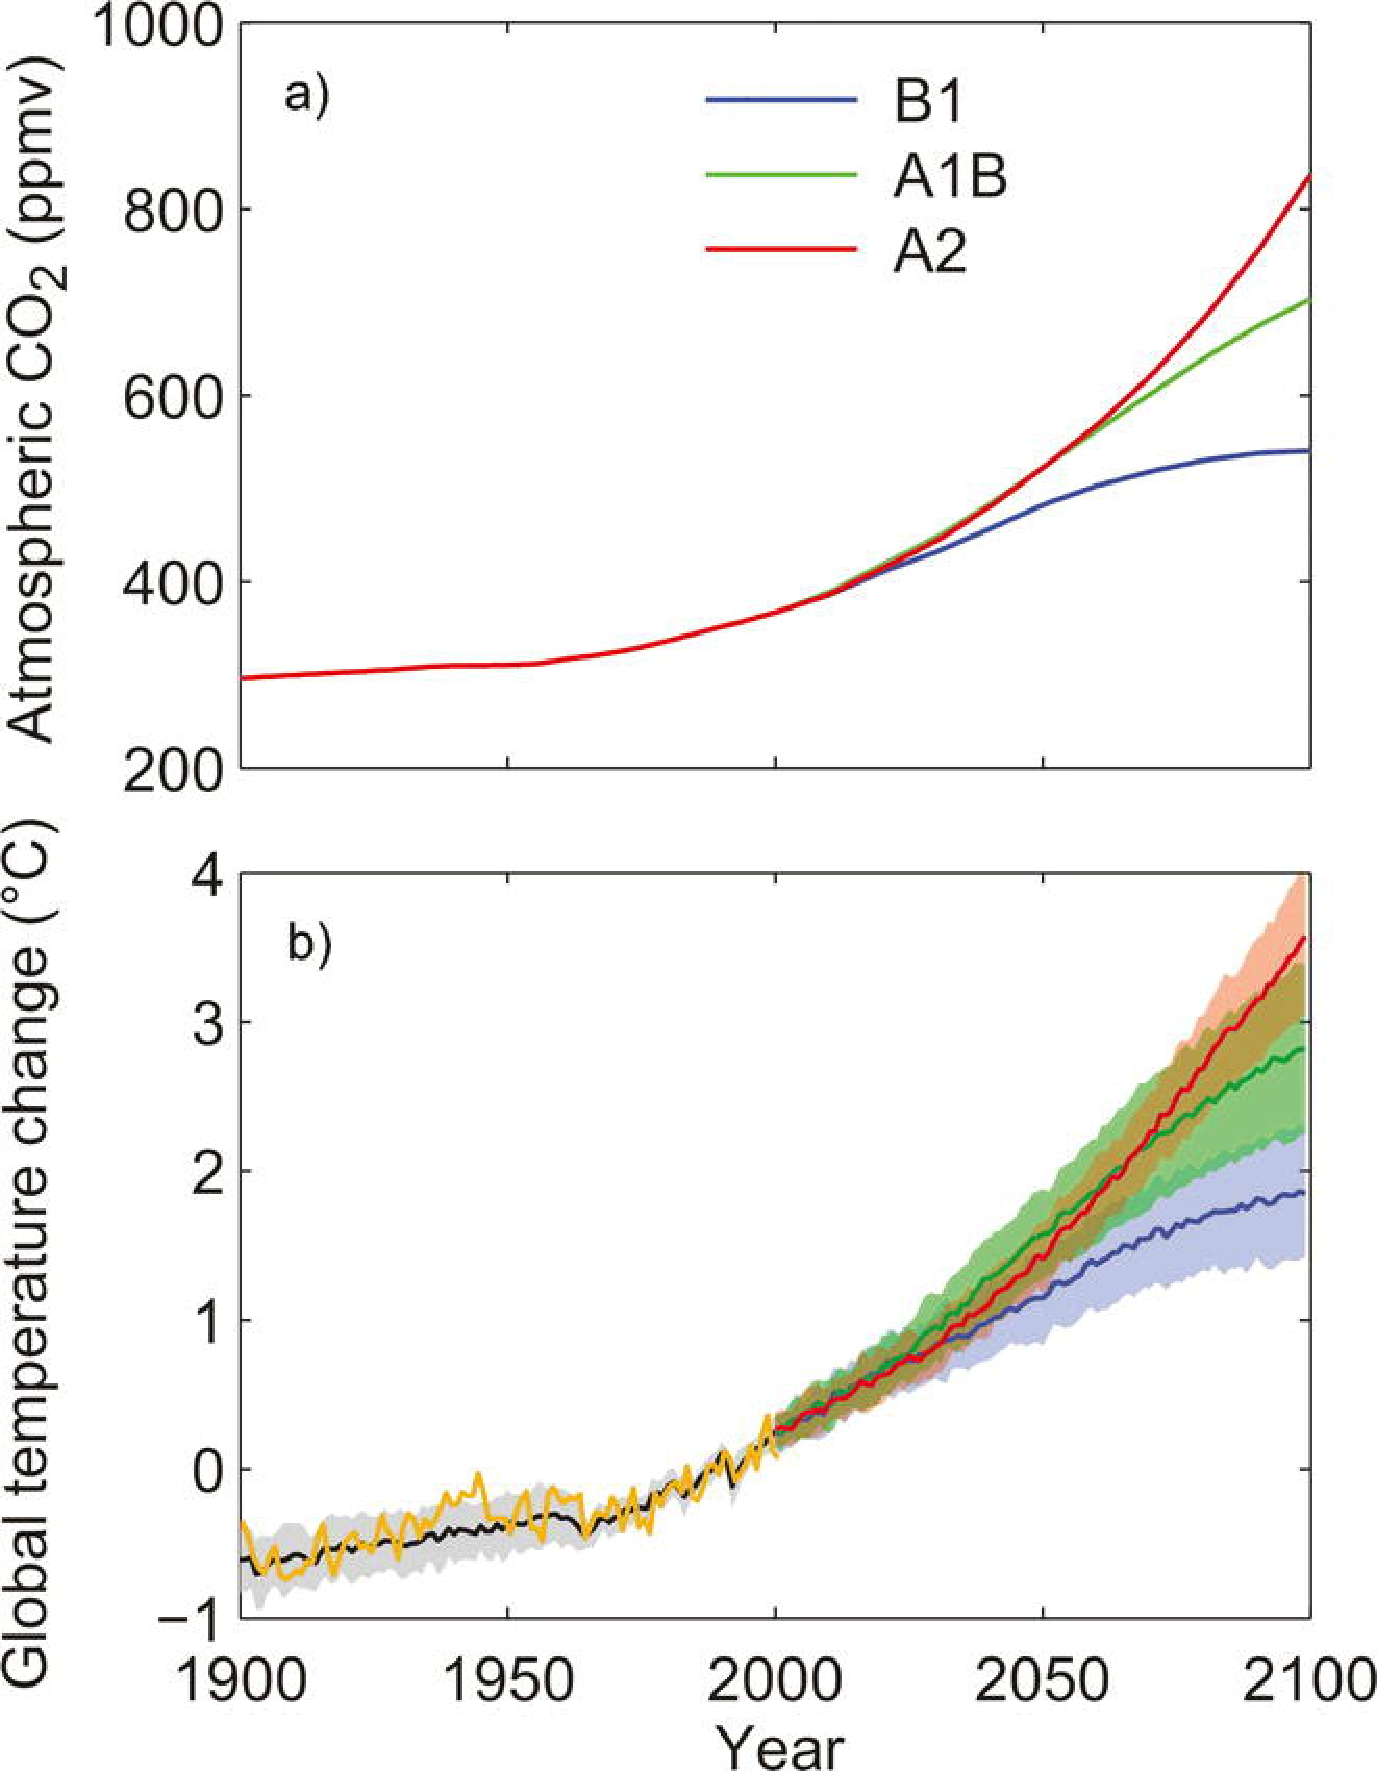
\includegraphics[width=19pc,angle=0]{figure01.pdf}\\
%  \caption{Enter the caption for your figure here.  Repeat as
%  necessary for each of your figures. Figure from \protect\cite{Knutti2008}.}\label{f1}
%\end{figure}

\end{document}